%----- Moritz:

%- Wie kommt man an die Gewichte der Events? -> data driven bkg estimation

%- lost lepton  

\begin{frame}
  \frametitle{Data-driven background estimation}
  \begin{itemize}
    \item Use data instead of MC to get lower uncertainties
    \item Example: Use Z($\mu \mu$) + jets and replace muons with neutrinos
    \item Disadv.: $\mathcal{B}(Z \rightarrow \mu \mu) < \mathcal{B}(Z \rightarrow \nu \nu)$ increases stat. uncertainty 
  \end{itemize}
  \begin{figure}[H]
    \centering
    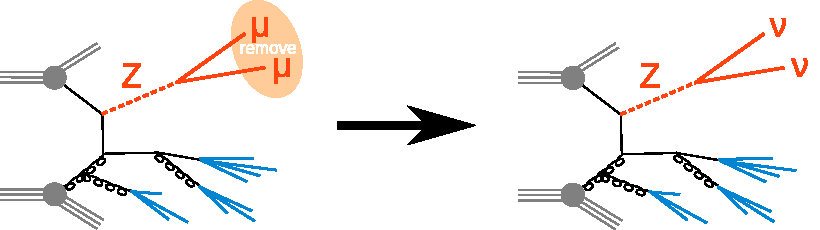
\includegraphics[width=0.8\textwidth]{figures/zmumu}
  \end{figure}
\end{frame}

\begin{frame}
  \frametitle{MC-only background estimation}
  \begin{figure}[H]
    \centering
    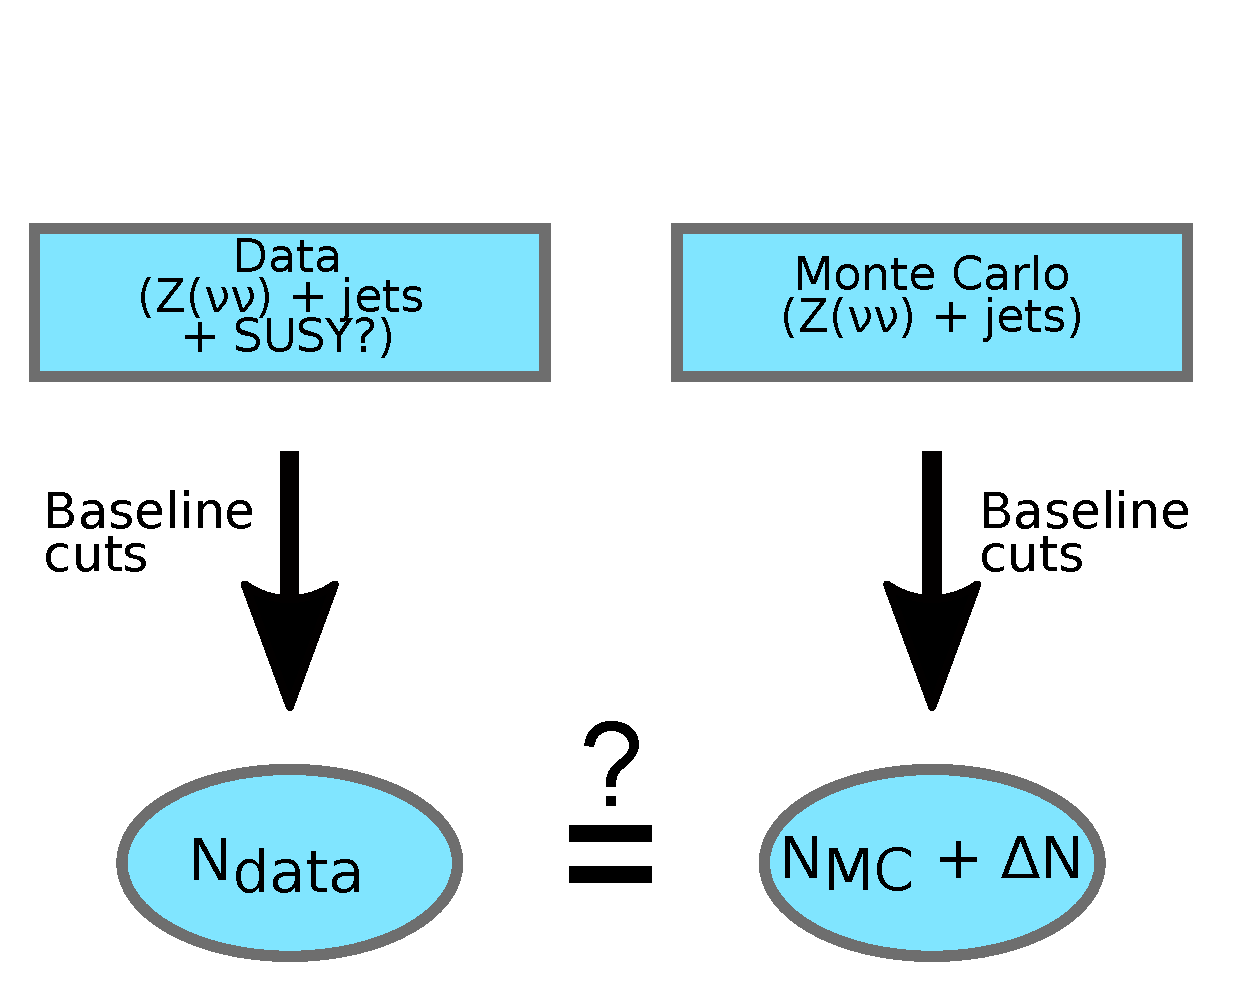
\includegraphics[width=0.7\textwidth,height=0.7\textheight,keepaspectratio]{figures/mc_znunu}
  \end{figure}
\end{frame}

\begin{frame}
  \frametitle{Data-driven background estimation (with Z($\mu\mu$))}
  \begin{figure}[H]
    \centering
    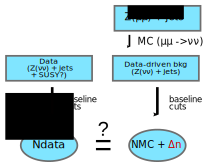
\includegraphics[width=0.8\textwidth,height=0.8\textheight,keepaspectratio]{figures/ddbe_zmumu}
  \end{figure}
\end{frame}

\begin{frame}
  \frametitle{Lost-lepton estimation}
  \begin{itemize}
    \item Lost leptons are electrons/muons not removed by lepton veto
    \item Reasons: Lepton not accepted, not well-reconstructed or not isolated
    \item Different approach is needed here: data-driven background estimation
  \end{itemize}

  \begin{figure}[H]
    \centering
     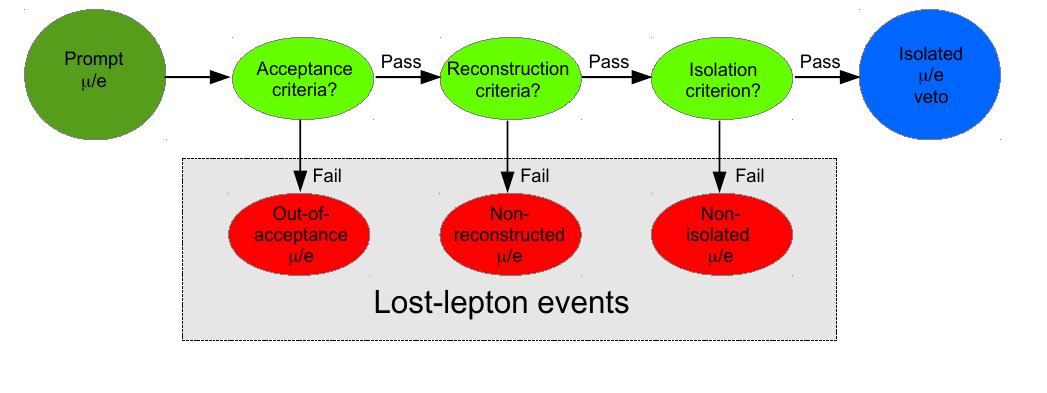
\includegraphics[width=\textwidth]{figures/lost-lepton.png}
    %\caption{aus Thesis}
  \end{figure}

\end{frame}

\begin{frame}
  \frametitle{Data-driven background estimation}
  \begin{itemize}
    \item Use lost-lepton probability $\omega(\alpha, \epsilon_{reco}, \epsilon_{iso})$ to get real number of events with leptons 
    \begin{itemize}
      \item $\alpha$: acceptance
      \item $\epsilon_{reco}$: reconstruction efficiency
      \item $\epsilon_{iso}$: isolation efficiency
    \end{itemize}
    \item Example: We observe 18 muons and know that 90\% of reconstructed muons are isolated
    \item $\rightarrow$ $N_\mu^{lost} = N_\mu^{iso} \cdot \frac{1 - \epsilon_{iso}}{\epsilon_{iso}} = 18 \cdot \frac{1 - 0.9}{0.9} = 2$
  \end{itemize}

\end{frame}
